\section{Aussagen}
\begin{center}
\begin{tabular}{l|c|c}
Aussage & w & f\\ \hline
Wasser ist nass & x & \\
A. Merkel ist Bundeskanzlerin & x & \\
Rößler wäre gern Bundeskanzler & ? & ?\\
Ein Kaninchen ist eine Pflanze & & x\\
Ein Dreieck hat vier Ecken & & x\\
Jede gerade Zahl größer 2 ist Summer zweier Primzahlen - Goldbach Vermutung & ? & ? \\
Wenn 2012 Frauenüberschuss bei Matheprofessorinen herrscht, dann ist die Erde eine Scheibe & x &\\
\end{tabular}

\quad\\
\quad\\

$ A \Rightarrow B$ ist wahr. \\
$A$ ist hinreichend für $B$. \\
$B$ ist notwendig für $A$. \\

\quad\\

\begin{tabular}{ll}
	$\neg A=$ nicht $A$ & $A \vee B =$ $A$ oder $B$\\
	$A \wedge B =$ $A$ und $B$ & $A \Leftrightarrow B =$ $A$ ist äquivalent zu $B$\\
\end{tabular}

\quad\\
\quad\\

\begin{tabular}{cc||ccccc}
$A$ & $B$ & $\neg A$ & $A \wedge B$ & $A \vee B$ & $A \Rightarrow B$ & $A \Leftrightarrow B$\\ \hline
w & w & f & w & w & w & w \\
w & f & f & f &w & f & f \\
f & w & w & f & w & w & f \\
f & f & w & f & f & w & w\\
\end{tabular}
\end{center}
%
%
%
\subsection{Satz:}
$A,B,C$ Folgende Aussagen sind wahr $\Rightarrow$ "`Tautologie"'
\begin{center}
\begin{tabular}{cc||ccc}
$A$ & $\neg A$ & $A \vee \neg A$ & $\neg(A\vee \neg A)$ & $\neg(\neg A)$\\ \hline
w & f & w & w & w\\
f & w & w & w & f\\
\end{tabular}
\end{center}
\quad\\
\begin{enumerate}
\item $A\vee(\neg A)$
\item $\neg (A \wedge \neg A)$
\item $\neg (\neg A)$
\item $\neg (A \wedge B) \Leftrightarrow \neg A \neg B$ \ z.B. $A=$ Die Sonne scheint \ $B=$ Es ist bewölkt
\item $\neg (A \vee B) \Leftrightarrow \neg A \wedge \neg B$ \ z.B. $A=$ Wasser ist trocken \ $B=$ Es ist Sommer
\item $(A\Rightarrow B) \Leftrightarrow (\neg A \Rightarrow \neg B)$ \ $A=$ Es blitzt \ $B=$ es donnert
\item $A \wedge (A \Rightarrow B) \Rightarrow B$
\item $A \Rightarrow B \wedge \neg B \Rightarrow \neg A$
\item $[(A\Rightarrow B) \wedge(B\Rightarrow C)]\Rightarrow(A\Rightarrow C)$
\item $A\wedge (B\vee C)\Rightarrow (A\wedge B)\vee(A\wedge C)$
\item $A \vee(B\wedge C) \Rightarrow (A\vee B) \wedge (A \vee C)$
\end{enumerate}
4 und 5 sind die De Morgan'sche Gesetze. 7 Ist der Modus ponens, 8 Modus tollens und die 9 Modus barbara (=Transitivität)\\
%
%
%
\section{Mengen}
\subsection{Definition: (Cantor)}
Unter einer Menge verstehen wir jede Zusammenfassung von stemmten auch wohl unterscheidenen Objekten unserer Anschauungen oder unseren Denkens zu einem Ganzen\\

\begin{figure} [H]
\centering 
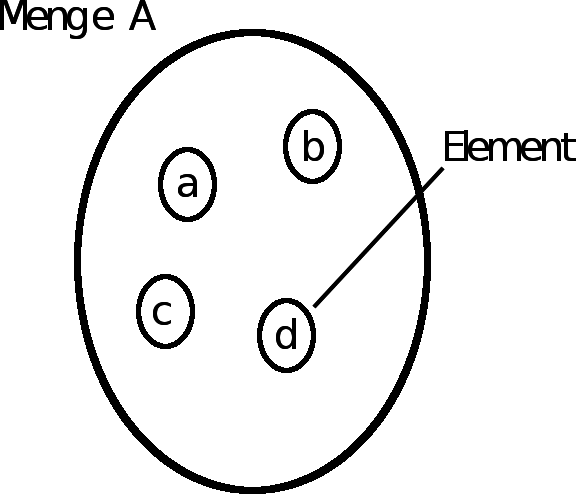
\includegraphics[width=4cm, height=3cm]{mainmatter/chapter0/pics/menge.png}
\caption{Eine einfache Menge} 
\end{figure}
\begin{equation*}
a \in A \qquad a \notin A \Leftrightarrow \neg (a \in A)
\end{equation*}
%
\subsection{Definition:}
$A, B$ Mengen 
\begin{enumerate}
\item $A \subset B \qquad \forall x \in A \Rightarrow x \in B$
\item $A \subsetneqq B \qquad (A \subset B) \wedge (A \neq B)$
\item $A = B \qquad A\subset B, \quad B\subset A$
\item $\emptyset \qquad \emptyset \subset A \quad \forall$ Mengen $A$
\item $|A| = \#A$ \qquad Anzahl der Elemente\\
 $|A| < \infty \qquad A=\{a_{1}, a_{2}, \dotsc, a_{n}\}$
\end{enumerate}
%
\textbf{Bemerkung:} \{1,2,1\} = \{1.2\}\\
\textbf{Beispiel:} \{1,2,\{1,2\},\{1,2\{1,3\}\}\}\\
gegeben Menge $M$, \quad $A=\{x \in M|x$ spricht italienisch\} = \{$x|(x \in M) \wedge x$ spricht italienisch\}